\documentclass[12pt]{article}

%%%%%% Packages
\usepackage{amsmath, amssymb}
\usepackage{graphicx}
\usepackage{bbm}


%%%%%% New commands
% iid text above the distribution sign
\newcommand{\iid}{\overset{\mathrm{\mathrm{iid}}}{\sim}}
% Expectation symbol
\DeclareMathOperator*{\E}{\mathbb{E}}
% Partial differentiation shorthand
\newcommand{\dpart}[2]{\frac{\partial #1}{\partial #2}}


%%%%%% Opening details
\title{Ito Integral}
\author{Treacher}


\begin{document}

\date{}
\maketitle

\begin{abstract}

\noindent Just some notes about the Ito integral, along with some preliminary information about Riemann and Riemann-Stieltjes integration. Summarised from various places online, including but not limited to:
\begin{itemize}
	\item https://www.youtube.com/watch?v=vHn1M6pUAWg
	\item http://www.columbia.edu/~ks20/FE-Notes/4700-07-Notes-Ito.pdf
\end{itemize}

\end{abstract}

\section{Preliminaries}
\subsection{Riemann integration}
For a regular non-stochastic function (black line in figure \ref{fig:riemannSums}), you can use Riemann integration to approximate the integral. This approach involves:
\begin{itemize}
	\item Divide range of integration into set of subintervals $P=\{t_0,t_1,t_2,...,t_n\}$
	\item Over all subintervals, calculate the lower and upper Riemann sums which represent the areas of the rectangles of width equal to the subinterval, and heights equal to the minimum and maximum function value in that interval (see figure \ref{fig:riemannSums}):
	\begin{itemize}
		\item Lower sum: $L = \sum_{i=1}^{n}\mathrm{min}\{f(t_i)\}\cdot(t_i-t_{i-1})$
		\item Upper sum: $U = \sum_{i=1}^{n}\mathrm{max}\{f(t_i)\}\cdot(t_i-t_{i-1})$
	\end{itemize}
	\item For a given function and a small number of partitions, the lower sum will be smaller than the upper sum.
	\item As the number of partitions increases, the values of the two sums will converge toward eachother (if the integral exists).
	\item When the values of the sums intersect, that value is taken to be the Riemann integral of that function over the relevant limits.
\end{itemize}

\begin{figure}[h!]
	\centering
	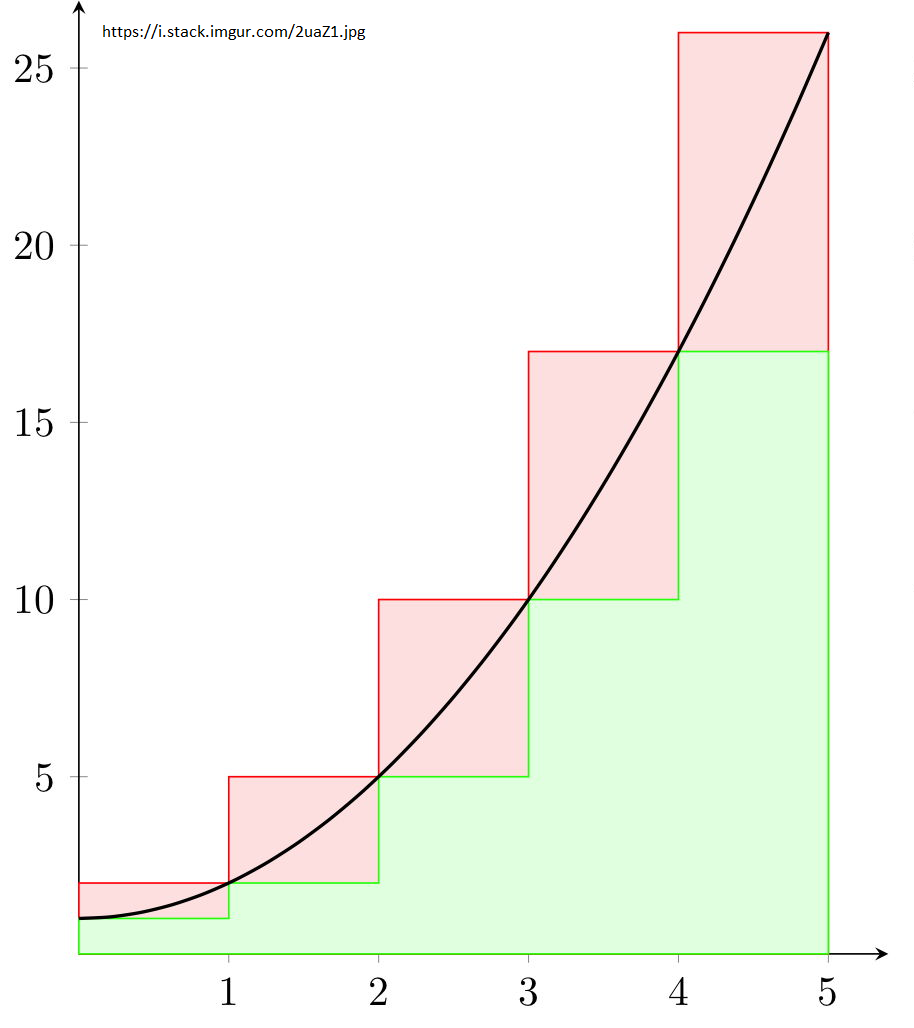
\includegraphics[width=0.8\linewidth]{riemannSums.png}
	\caption{Lower (green) and upper (red) Riemann sums of a function (black)}
	\label{fig:riemannSums}
\end{figure}

\subsection{Riemann-Stieltjes integration}

This is a generalisation of Riemann integration, but where Riemann uses fixed subintervals of $(t_i-t_{i-1})$ as the integrator (d$t$), the Stieltjes approach uses a monotonic function instead.\\
\\
Now the analogous lower and upper sums are:
\begin{eqnarray}
	L &= \sum_{i=1}^{n}\mathrm{min}\{f(t_i)\}\cdot(g(t_i)-g(t_{i-1}))\\
	U &= \sum_{i=1}^{n}\mathrm{max}\{f(t_i)\}\cdot(g(t_i)-g(t_{i-1}))
\end{eqnarray}
\noindent where $g(t_i)>g(t_{i-1})$ when $t_i>t_{i-1}$\\
\\
Imagine a 3D plot of $f(t)$ vs $g(t)$ vs $t$ such as in  figure \ref{fig:stieltjesIntegration}.
\begin{figure}[h!]
	\centering
	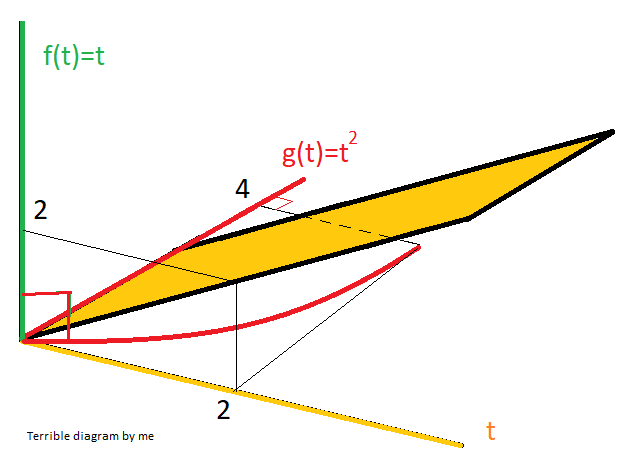
\includegraphics[width=0.8\linewidth]{stieltjesIntegration.png}
	\caption{Stieltjes framework with the integrand $f(t)=t$ and integrator $g(t)=t^2$.}
	\label{fig:stieltjesIntegration}
\end{figure}

\noindent The lower sum will be the value of $f(t=0)=0$ multiplied by the corresponding change in value of $g(t)$. This will be zero. The upper sum will be the max value of $f(t)$ over the range of $[0,2]$ which is $f(2)=2$ multiplied by the change in value of integrator: $g(t_i)-g(t_{i-1})=2^2 - 0^2=4$, giving a final result of 8.\\
\\
Same logic as above applies when increasing the number of partitions until the upper and lower sums intersect, which represents the value of the integral (if it exists). Note that when adding more partitions, the should be placed at equally spaced values of the integrator $g(t)$. In this example with $g(t)=t^2$, the half way point would be half the max value of $g(t)$ which is 4, evaluated at the corresponding value of $t$. This would be $t=\sqrt{2}$.


\section{Brownian motion as integrator}

\subsection{Riemann-Stieltjes approach}
The above Stieltjes approach doesn't translate to using Brownian motion as the integrator because of its fractal and zig-zagy nature. These factors make proofs of convergence difficult and motivate the choice for a different kind of integration: One using `simple functions'.\\
\\
More formally, if you were to try and integrate standard brownian motion as
\begin{equation}
	\int_{0}^{t}B_s\mathrm{d}B_s
\end{equation}

\noindent you would partition the integral into the $n$ relevant subintervals and try to find the Riemann-Stieltjes sums:
\begin{eqnarray}
	S^1_n(t) =& \sum_{i=1}^{n}B(t_{i-1})\cdot(B(t_i)-B(t_{i-1}))\\
	S^2_n(t) =& \sum_{i=1}^{n}B(t_i)\cdot(B(t_i)-B(t_{i-1}))
\end{eqnarray}

\noindent Now if the Riemann-Stieltjes integral exists, $S^1_n(t)-S^2_n(t)\to 0$ as the largest subinterval shrank to zero: max$\{t_i-t_{i-1}\}\to 0$. But multiplying out the argument of the sums above, and observing that disjoint time interval brownian terms are independent hence multiply to zero, we see
\begin{equation}
	S^1_n(t)-S^2_n(t)=\sum_{i=1}^{n}\left(B_{t_i}-B_{t_{i-1}}\right)^2 > 0
\end{equation}

\noindent and as shown in the quadraticVariation folder, the expectation of $B_{t_i}-B_{t_{i-1}}$ is $t_i-t_{i-1}$, the sum of which is just equal to the time horizon $t$:

\begin{equation}
	\E\left[S^1_n(t)-S^2_n(t)\right]=\sum_{i=1}^{n}t_i-t_{i-1}=t\neq0
\end{equation}

\noindent meaning that the sums don't converge, and the Riemann-Stieltjes integral does not exist for a Brownian motion process.

\subsection{Simple functions approach}

Basic steps:
\begin{itemize}
	\item Replace the function $f$ with a constant. Set the value as the average of $f$ between the relevant limits
	\item Now the integral of the new constant function with respect to the Brownian integrator is just the constant value multiplied by the change in the Brownian over that the interval.
	\item Now make subintervals by splitting the constant valued function into multiple regions of constant values (each constant is just the average of the function in that region)
	\item As the number of subintervals becomes large, you end up with a series of step functions that approximate the level of the function (see figure \ref{fig:quantPieScreenShot}).
	\item The limiting value as the number of subintervals $\to\infty$ is the Ito's integral value.
\end{itemize}

\noindent Proofs of convergence of the Ito integral depend on convergence in the mean squared sense which for a stochastic process $X_n$ and terminal value $X$ is defined as

\begin{equation}
	\lim\limits_{n\to\infty}\E\left[\left|X_n - X\right|^2\right]=0
\end{equation}

\noindent To test the convergence of the Ito integral approach, you use the Cauchy convergence or Cauchy criteria test: For every $\epsilon>0$, $\exists\,N$ such that $\forall\,n>N, n>M:$ $\left|X_n-X_m\right|<\epsilon$. This is essentially saying that for large enough values of $n,m$, terms $n,m$ of the process will converge to within a distance of $\epsilon$, allowing the mean squared convergence to be recast as

\begin{equation} \label{eq:meanSquaredCauchy}
	\lim\limits_{n,m\to\infty}\E\left[\left|X_n - X_m\right|^2\right]=0
\end{equation}

\noindent Useful because we can prove convergence without knowing the limit $X$.\\
\\
Now the expectation is just a probability weighted sum, allowing us to write the above in terms of the L$_2$ norm:

\begin{equation}
	\lim\limits_{n,m\to\infty}||X_n-X_m||^2_{L_2}=0
\end{equation}

\begin{figure}[h!]
	\centering
	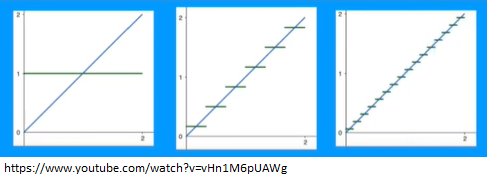
\includegraphics[width=\linewidth]{quantPieScreenShot.png}
	\caption{Simple functions (green) approximations to a function (blue) with an increasing number of subintervals (left to right).}
	\label{fig:quantPieScreenShot}
\end{figure}

\noindent The sequence of subintervals can be written as

\begin{eqnarray}\label{eq:simpleFunctionIndicator}
	S(t)=\sum_{i=1}^{n}c_i\cdot\mathbbm{1}_{t_{i-1}, t_i}
\end{eqnarray}

\noindent where $c_i$ are the simple function values and $\mathbbm{1}_{t_{i-1}, t_i}$ is the indicator variable that is = 1 between ${t_{i-1}, t_i}$ and 0 everywhere else.\\
\\
The $c_i$s in the above are there to approximate the function $f$. As a technicality, we say that the $c_i$s are `adapted to the filtration $F$' which roughly means that at a given time $t$, only the values of $c_i$ with $i\leq t_{i-1}$ are available implying we can't see into the future.\\
\\
From equation \ref{eq:simpleFunctionIndicator}, we can write the ito integral as the sum of simple (constant) functions over subintervals:

\begin{equation}
	I(t)=\sum_{i=1}^{n}c_i\cdot\left(B_{t_i}-B_{t_{i-1}}\right)
\end{equation}






\section{Summary}

So we started with trying to calculate the integral of some function with respect to a stochastic Brownian integrator:

\begin{equation}
	I(f)=\int_{0}^{t}f(u,B_u)\,\mathrm{d}B_u.
\end{equation}

\noindent Regular Riemann or Riemann-Stieltjes approached don't work because of the details of how the Brownian motion is put together.\\
\\
Next step was to approximate the integral as a limit of a sum of simple functions $c_i$ which locally approximate the value(s) of $f$:

\begin{equation}
	S(t)=\sum_{i=1}^{n}c_i\cdot\mathbbm{1}_{t_{i-1}, t_i}
\end{equation}

\noindent From there, we define the Ito integral as the limiting value of a sum:

\begin{equation}
	I(t)=\sum_{i=1}^{n}c_i\cdot\left(B_{t_i}-B_{t_{i-1}}\right)
\end{equation}


\noindent so for completeness, the \textbf{Ito integral} is:

\begin{equation}
	\int_{0}^{t}f(u,B_u)\,\mathrm{d}B_u\approx\sum_{i=1}^{n}f_i\cdot\left(B_{t_i}-B_{t_{i-1}}\right)
\end{equation}
\noindent where I've replaced $c_i$ with $f_i$ to emphasize the approximation.\\
\\
The proof of convergence is done via the Cauchy criteria and is somewhat involved. Check the youtube link in the abstract for a decent walkthrough.

\end{document}